\documentclass{beamer}
\usetheme{Madrid}
\usepackage[utf8]{inputenc}
\usepackage{default}
\usepackage{tkz-graph}

\tikzset{
  LabelStyle/.style = { rectangle, rounded corners, draw,
                       font = \bfseries },
  EdgeStyle/.append style = {-} }
\title{Latency optimization for C-RAN}

\author{M.~Guiraud }


\institute[Nokia Bell Labs, UVSQ] 
{
  Nokia Bell Labs France - 
  Universit\'e de Versailles Saint Quentin\\
}

\subject{Theoretical Computer Science}

\begin{document}

\begin{frame}
  \titlepage
\end{frame}


\begin{frame}{Context}
  \centering
  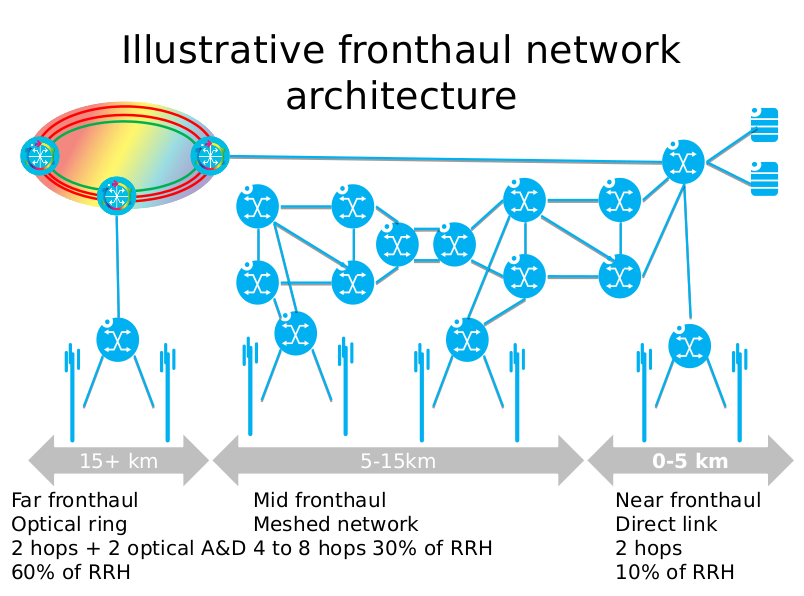
\includegraphics[scale=0.38]{fronthaul0.png}
\end{frame}

\begin{frame}{Context}
  \centering
  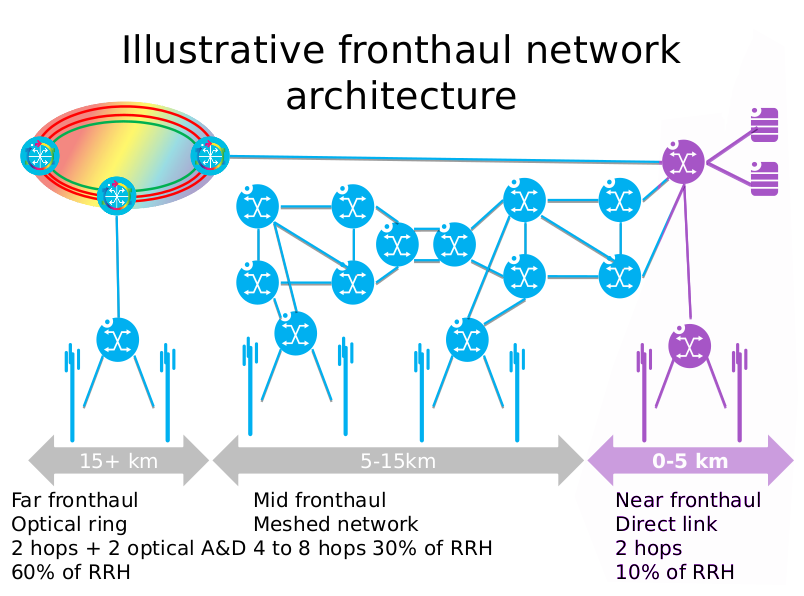
\includegraphics[scale=0.38]{fronthaul.png}
\end{frame}


\begin{frame}{Problem}
  \centering
  
\scalebox{0.5}{
\begin{tikzpicture}
  \SetGraphUnit{5}
  \Vertex[x=0,y=0]{RRH 3}
  \Vertex[x=0,y=4]{RRH 2}
  \Vertex[x=0,y=8]{RRH 1}
  
  \Vertex[x=16,y=0]{BBU 3}
  \Vertex[x=16,y=4]{BBU 2}
  \Vertex[x=16,y=8]{BBU 1}
  
  \Vertex[x=4,y=4]{Switch 1}
  \Vertex[x=12,y=4]{Switch 2}  
  \tikzset{
  EdgeStyle/.append style = {green} }
  \Edge[label = $a_1$](BBU 1)(Switch 2)
  \Edge[label = $b_1$](Switch 1)(RRH 1)
  
  \tikzset{
  EdgeStyle/.append style = {blue} }
  \Edge[label = $a_2$](BBU 2)(Switch 2)
  \Edge[label = $b_2$](Switch 1)(RRH 2)
  
  \tikzset{
  EdgeStyle/.append style = {red} }
  \Edge[label = $a_3$](BBU 3)(Switch 2)
  \Edge[label = $b_3$](Switch 1)(RRH 3)
  
  \tikzset{
  EdgeStyle/.append style = {black} }
  \Edge(Switch 1)(Switch 2)

\end{tikzpicture}
}

  Scheduling the messages
  \begin{itemize}
   \item No collisions on switches
   \item Periodicity
  \end{itemize}

 
\end{frame}

\begin{frame}{Problem}
  \centering
  
\scalebox{0.5}{
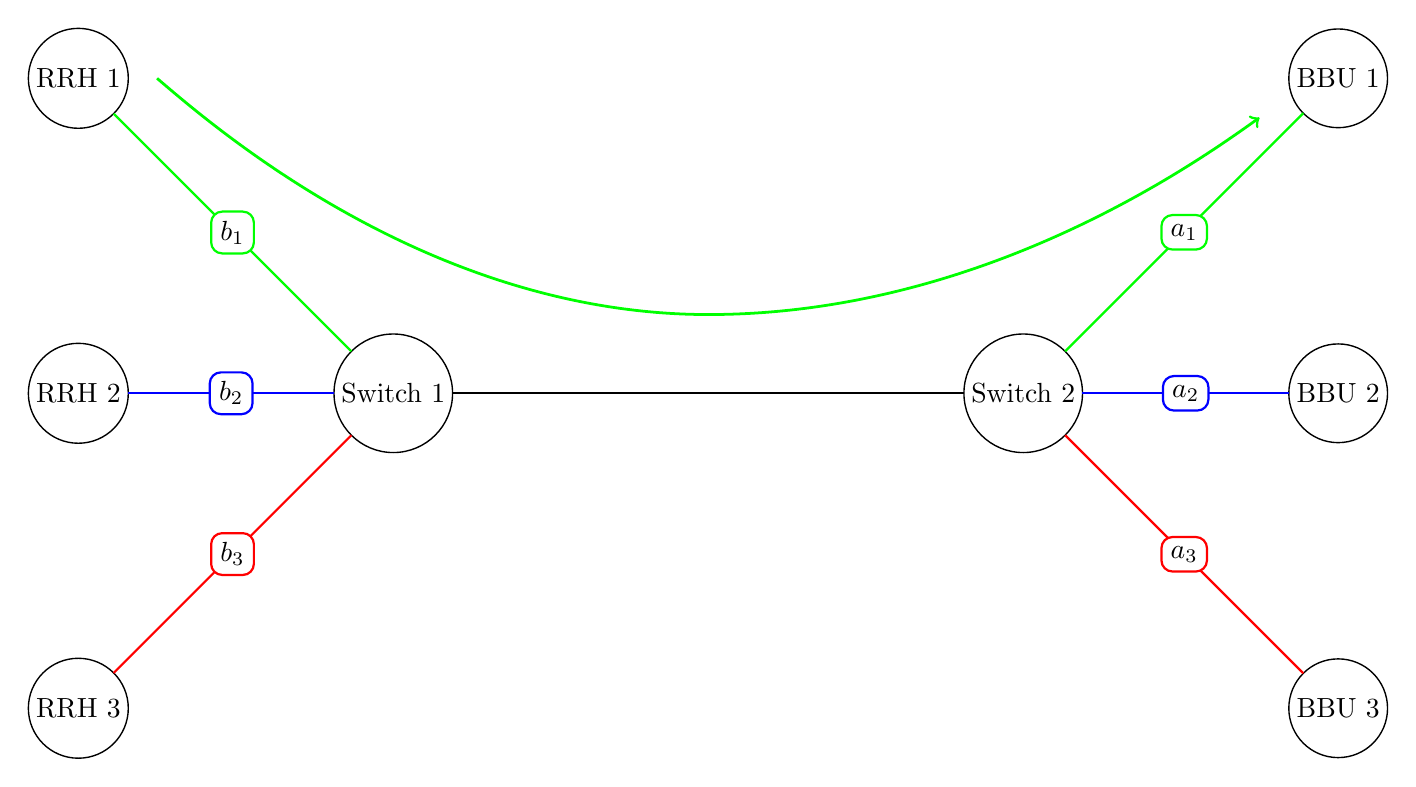
\begin{tikzpicture}
  \SetGraphUnit{5}
  \Vertex[x=0,y=0]{RRH 3}
  \Vertex[x=0,y=4]{RRH 2}
  \Vertex[x=0,y=8]{RRH 1}
  
  \Vertex[x=16,y=0]{BBU 3}
  \Vertex[x=16,y=4]{BBU 2}
  \Vertex[x=16,y=8]{BBU 1}
  
  \Vertex[x=4,y=4]{Switch 1}
  \Vertex[x=12,y=4]{Switch 2}  
  \tikzset{
  EdgeStyle/.append style = {green} }
  \Edge[label = $a_1$](BBU 1)(Switch 2)
  \Edge[label = $b_1$](Switch 1)(RRH 1)
  
  \tikzset{
  EdgeStyle/.append style = {blue} }
  \Edge[label = $a_2$](BBU 2)(Switch 2)
  \Edge[label = $b_2$](Switch 1)(RRH 2)
  
  \tikzset{
  EdgeStyle/.append style = {red} }
  \Edge[label = $a_3$](BBU 3)(Switch 2)
  \Edge[label = $b_3$](Switch 1)(RRH 3)
  
  \tikzset{
  EdgeStyle/.append style = {black} }
  \Edge(Switch 1)(Switch 2)

  \draw[->,line width=1pt,green] (1,8) parabola bend (8,5) (15,7.5);


\end{tikzpicture}
}

RRH $\rightarrow$ BBU
\end{frame}



\begin{frame}{Problem}
  \centering
  
\scalebox{0.5}{
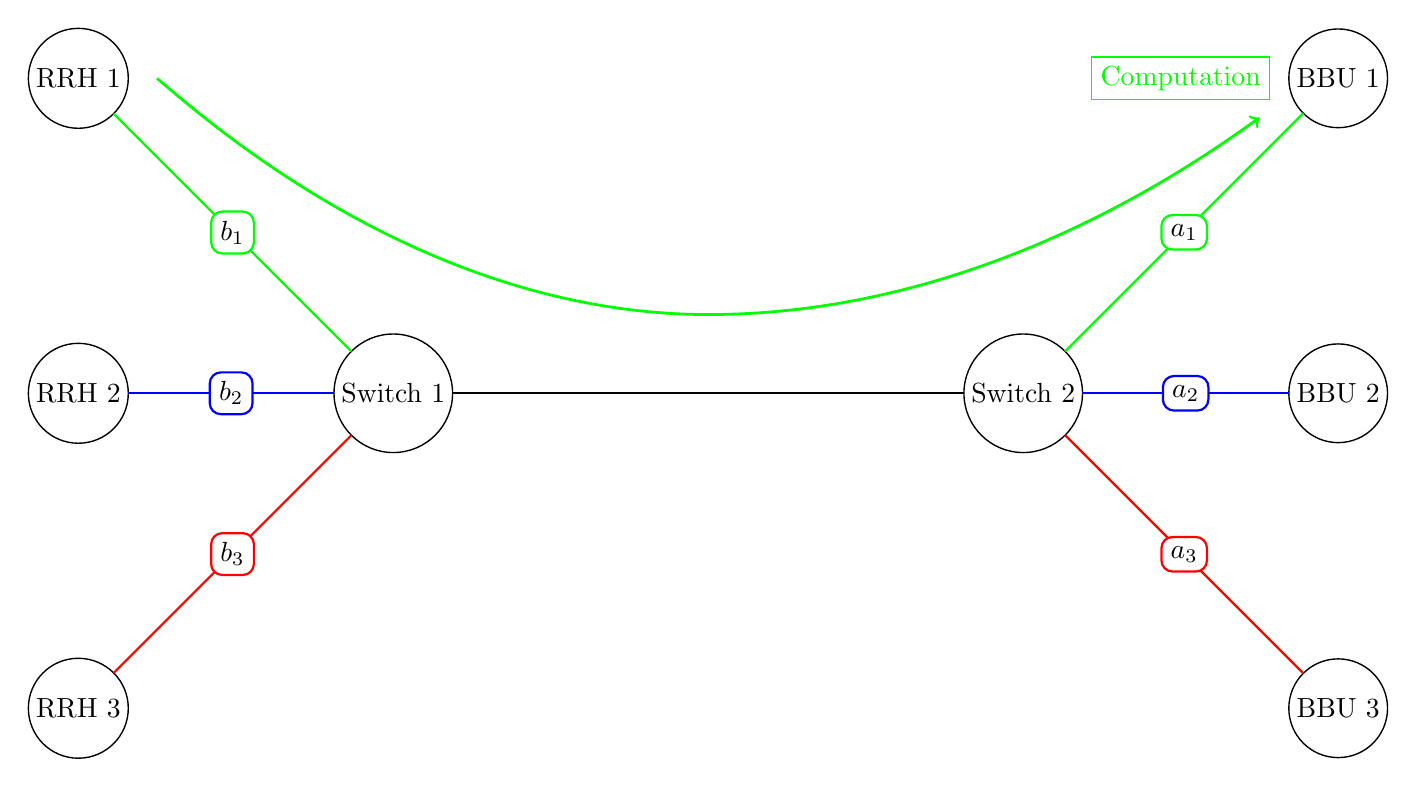
\begin{tikzpicture}
  \SetGraphUnit{5}
  \Vertex[x=0,y=0]{RRH 3}
  \Vertex[x=0,y=4]{RRH 2}
  \Vertex[x=0,y=8]{RRH 1}
  
  \Vertex[x=16,y=0]{BBU 3}
  \Vertex[x=16,y=4]{BBU 2}
  \Vertex[x=16,y=8]{BBU 1}
  
  \Vertex[x=4,y=4]{Switch 1}
  \Vertex[x=12,y=4]{Switch 2}  
  \tikzset{
  EdgeStyle/.append style = {green} }
  \Edge[label = $a_1$](BBU 1)(Switch 2)
  \Edge[label = $b_1$](Switch 1)(RRH 1)
  
  \tikzset{
  EdgeStyle/.append style = {blue} }
  \Edge[label = $a_2$](BBU 2)(Switch 2)
  \Edge[label = $b_2$](Switch 1)(RRH 2)
  
  \tikzset{
  EdgeStyle/.append style = {red} }
  \Edge[label = $a_3$](BBU 3)(Switch 2)
  \Edge[label = $b_3$](Switch 1)(RRH 3)
  
  \tikzset{
  EdgeStyle/.append style = {black} }
  \Edge(Switch 1)(Switch 2)

  \draw[->,line width=1pt,green] (1,8) parabola bend (8,5) (15,7.5);
  \node[draw,green] at (14,8) {Computation};



\end{tikzpicture}
}

Computation time
\end{frame}



\begin{frame}{Problem}
  \centering
  
\scalebox{0.5}{
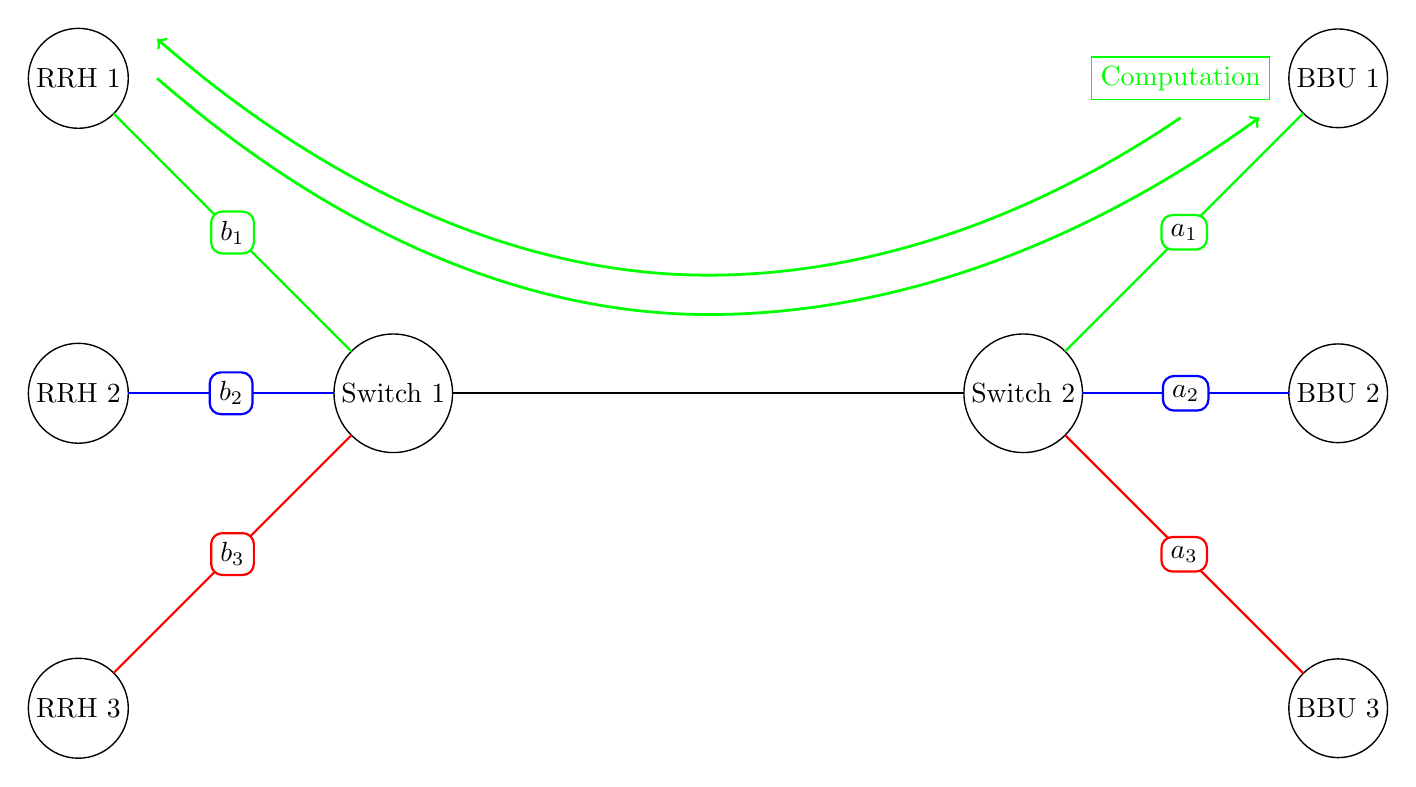
\begin{tikzpicture}
  \SetGraphUnit{5}
  \Vertex[x=0,y=0]{RRH 3}
  \Vertex[x=0,y=4]{RRH 2}
  \Vertex[x=0,y=8]{RRH 1}
  
  \Vertex[x=16,y=0]{BBU 3}
  \Vertex[x=16,y=4]{BBU 2}
  \Vertex[x=16,y=8]{BBU 1}
  
  \Vertex[x=4,y=4]{Switch 1}
  \Vertex[x=12,y=4]{Switch 2}  
  \tikzset{
  EdgeStyle/.append style = {green} }
  \Edge[label = $a_1$](BBU 1)(Switch 2)
  \Edge[label = $b_1$](Switch 1)(RRH 1)
  
  \tikzset{
  EdgeStyle/.append style = {blue} }
  \Edge[label = $a_2$](BBU 2)(Switch 2)
  \Edge[label = $b_2$](Switch 1)(RRH 2)
  
  \tikzset{
  EdgeStyle/.append style = {red} }
  \Edge[label = $a_3$](BBU 3)(Switch 2)
  \Edge[label = $b_3$](Switch 1)(RRH 3)
  
  \tikzset{
  EdgeStyle/.append style = {black} }
  \Edge(Switch 1)(Switch 2)

  \draw[->,line width=1pt,green] (1,8) parabola bend (8,5) (15,7.5);
  \node[draw,green] at (14,8) {Computation};
  \draw[<-,line width=1pt,green] (1,8.5) parabola bend (8,5.5) (14,7.5);


\end{tikzpicture}
}

BBU $\rightarrow$ RRH
\end{frame}


\begin{frame}{Tools}
  \centering
  
\scalebox{0.5}{
\begin{tikzpicture}
  \SetGraphUnit{5}
  \Vertex[x=0,y=0]{RRH 3}
  \Vertex[x=0,y=4]{RRH 2}
  \Vertex[x=0,y=8]{RRH 1}
  
  \Vertex[x=16,y=0]{BBU 3}
  \Vertex[x=16,y=4]{BBU 2}
  \Vertex[x=16,y=8]{BBU 1}
  
  \Vertex[x=4,y=4]{Switch 1}
  \Vertex[x=12,y=4]{Switch 2}  
  \tikzset{
  EdgeStyle/.append style = {green} }
  \Edge[label = $a_1$](BBU 1)(Switch 2)
  \Edge[label = $b_1$](Switch 1)(RRH 1)
  
  \tikzset{
  EdgeStyle/.append style = {blue} }
  \Edge[label = $a_2$](BBU 2)(Switch 2)
  \Edge[label = $b_2$](Switch 1)(RRH 2)
  
  \tikzset{
  EdgeStyle/.append style = {red} }
  \Edge[label = $a_3$](BBU 3)(Switch 2)
  \Edge[label = $b_3$](Switch 1)(RRH 3)
  
  \tikzset{
  EdgeStyle/.append style = {black} }
  \Edge(Switch 1)(Switch 2)

  \node (0) at (1,-1){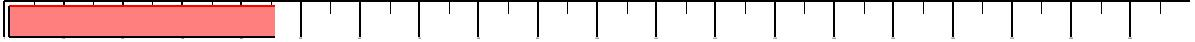
\includegraphics[scale=0.1]{chronogrames/0.jpeg}};
  \node (1) at (1,3){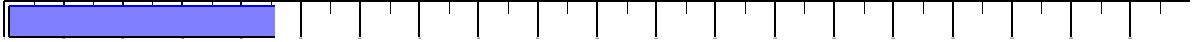
\includegraphics[scale=0.1]{chronogrames/1.jpeg}};
  \node (2) at (1,7){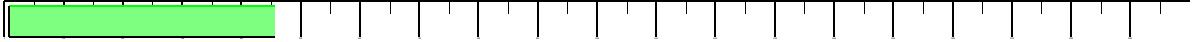
\includegraphics[scale=0.1]{chronogrames/2.jpeg}};
  \node (2) at (4,5){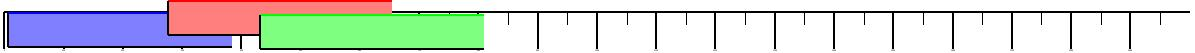
\includegraphics[scale=0.1]{chronogrames/3.jpeg}};
\end{tikzpicture}
}

\end{frame}


\begin{frame}{Tools}
  \centering
  
\scalebox{0.5}{
\begin{tikzpicture}
  \SetGraphUnit{5}
  \Vertex[x=0,y=0]{RRH 3}
  \Vertex[x=0,y=4]{RRH 2}
  \Vertex[x=0,y=8]{RRH 1}
  
  \Vertex[x=16,y=0]{BBU 3}
  \Vertex[x=16,y=4]{BBU 2}
  \Vertex[x=16,y=8]{BBU 1}
  
  \Vertex[x=4,y=4]{Switch 1}
  \Vertex[x=12,y=4]{Switch 2}  
  \tikzset{
  EdgeStyle/.append style = {green} }
  \Edge[label = $a_1$](BBU 1)(Switch 2)
  \Edge[label = $b_1$](Switch 1)(RRH 1)
  
  \tikzset{
  EdgeStyle/.append style = {blue} }
  \Edge[label = $a_2$](BBU 2)(Switch 2)
  \Edge[label = $b_2$](Switch 1)(RRH 2)
  
  \tikzset{
  EdgeStyle/.append style = {red} }
  \Edge[label = $a_3$](BBU 3)(Switch 2)
  \Edge[label = $b_3$](Switch 1)(RRH 3)
  
  \tikzset{
  EdgeStyle/.append style = {black} }
  \Edge(Switch 1)(Switch 2)

  \node (0) at (1,-1){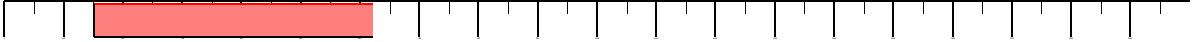
\includegraphics[scale=0.1]{chronogrames/4.jpeg}};
  \node (1) at (1,3){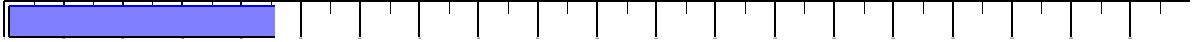
\includegraphics[scale=0.1]{chronogrames/1.jpeg}};
  \node (2) at (1,7){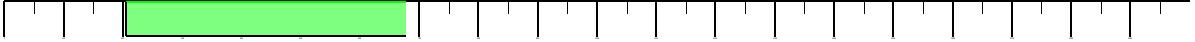
\includegraphics[scale=0.1]{chronogrames/5.jpeg}};
  \node (2) at (4,5){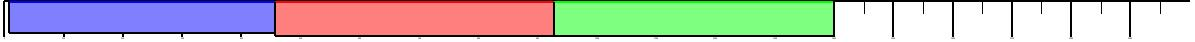
\includegraphics[scale=0.1]{chronogrames/6.jpeg}};
\end{tikzpicture}
}

Deterministic sending
\end{frame}


\begin{frame}{Tools}
  \centering
  
\scalebox{0.5}{
\begin{tikzpicture}
  \SetGraphUnit{5}
  \Vertex[x=0,y=0]{RRH 3}
  \Vertex[x=0,y=4]{RRH 2}
  \Vertex[x=0,y=8]{RRH 1}
  
  \Vertex[x=16,y=0]{BBU 3}
  \Vertex[x=16,y=4]{BBU 2}
  \Vertex[x=16,y=8]{BBU 1}
  
  \Vertex[x=4,y=4]{Switch 1}
  \Vertex[x=12,y=4]{Switch 2}  
  \tikzset{
  EdgeStyle/.append style = {green} }
  \Edge[label = $a_1$](BBU 1)(Switch 2)
  \Edge[label = $b_1$](Switch 1)(RRH 1)
  
  \tikzset{
  EdgeStyle/.append style = {blue} }
  \Edge[label = $a_2$](BBU 2)(Switch 2)
  \Edge[label = $b_2$](Switch 1)(RRH 2)
  
  \tikzset{
  EdgeStyle/.append style = {red} }
  \Edge[label = $a_3$](BBU 3)(Switch 2)
  \Edge[label = $b_3$](Switch 1)(RRH 3)
  
  \tikzset{
  EdgeStyle/.append style = {black} }
  \Edge(Switch 1)(Switch 2)

  \node (0) at (1,-1){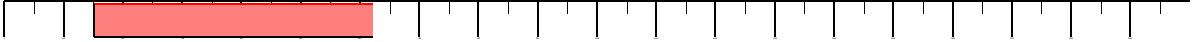
\includegraphics[scale=0.1]{chronogrames/4.jpeg}};
  \node (1) at (1,3){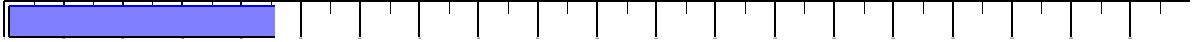
\includegraphics[scale=0.1]{chronogrames/1.jpeg}};
  \node (2) at (1,7){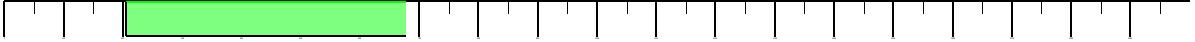
\includegraphics[scale=0.1]{chronogrames/5.jpeg}};
  \node (2) at (4,5){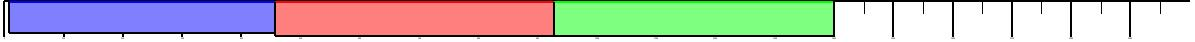
\includegraphics[scale=0.1]{chronogrames/6.jpeg}};
  \node (2) at (15,-1){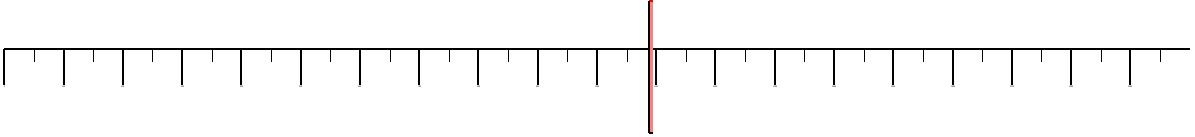
\includegraphics[scale=0.1]{chronogrames/7.jpeg}};
  \node (2) at (15,3){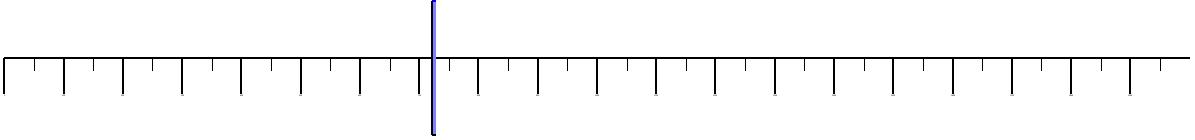
\includegraphics[scale=0.1]{chronogrames/8.jpeg}};
  \node (2) at (15,7){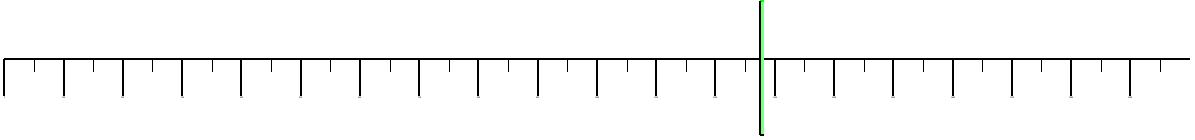
\includegraphics[scale=0.1]{chronogrames/9.jpeg}};
\end{tikzpicture}
}

Deterministic sending
\end{frame}

\begin{frame}{Inputs}


  \begin{tabular}{|c|c|}
  \hline
   Links capacity & 10Gbps \\
   \hline
   Flow/RRH & 1.228Gbps \\
   \hline
   Flow max ($l_{max}$) & 7 \\
   \hline
   Considered Range & 0-5km \\
   \hline
   Periodicity & 1ms \\
   \hline
   \end{tabular}
   
   Each links does have a delay in slots corresponding to it's transit time.\\

  The Flow values in slots correspond to the transmission time.\\

   \begin{tabular}{|c|c|}
   \hline
   Period & 19500 slots(1ms) \\
   \hline
   1 Flow & 2500 slots\\
   \hline
   Range & 2000 slots\\
   \hline
  \end{tabular}

  
  
\end{frame}


\begin{frame}{Trivial case}
\centering
\scalebox{0.5}{
  \begin{tikzpicture}
  \SetGraphUnit{5}
  \Vertex[x=0,y=0]{RRH 3}
  \Vertex[x=0,y=4]{RRH 2}
  \Vertex[x=0,y=8]{RRH 1}
  
  \Vertex[x=16,y=0]{BBU 3}
  \Vertex[x=16,y=4]{BBU 2}
  \Vertex[x=16,y=8]{BBU 1}
  
  \Vertex[x=4,y=4]{Switch 1}
  \Vertex[x=12,y=4]{Switch 2}
    
  \tikzset{
  EdgeStyle/.append style = {green} }
  \Edge[label = 0](BBU 1)(Switch 2)
  \Edge[label = $b_1$](Switch 1)(RRH 1)
  
  \tikzset{
  EdgeStyle/.append style = {blue} }
  \Edge[label = 0](BBU 2)(Switch 2)
  \Edge[label = $b_2$](Switch 1)(RRH 2)
  
  \tikzset{
  EdgeStyle/.append style = {red} }
  \Edge[label = 0](BBU 3)(Switch 2)
  \Edge[label = $b_3$](Switch 1)(RRH 3)
  
  \tikzset{
  EdgeStyle/.append style = {black} }
  \Edge(Switch 1)(Switch 2)
\end{tikzpicture}
}

  \begin{itemize}
  \item Scheduling all messages following each others
  \item No waiting times
  \end{itemize}
\end{frame}


\begin{frame}{Harder case}
\centering
\scalebox{0.5}{
\begin{tikzpicture}
  \SetGraphUnit{5}
  \Vertex[x=0,y=0]{RRH 3}
  \Vertex[x=0,y=4]{RRH 2}
  \Vertex[x=0,y=8]{RRH 1}
  
  \Vertex[x=16,y=0]{BBU 3}
  \Vertex[x=16,y=4]{BBU 2}
  \Vertex[x=16,y=8]{BBU 1}
  
  \Vertex[x=4,y=4]{Switch 1}
  \Vertex[x=12,y=4]{Switch 2}
  
  
  \tikzset{
  EdgeStyle/.append style = {green} }
  \Edge[label = $a_1$](BBU 1)(Switch 2)
  \Edge[label = 0](Switch 1)(RRH 1)
  
  \tikzset{
  EdgeStyle/.append style = {blue} }
  \Edge[label = $a_2$](BBU 2)(Switch 2)
  \Edge[label = 0](Switch 1)(RRH 2)
  
  \tikzset{
  EdgeStyle/.append style = {red} }
  \Edge[label = $a_3$](BBU 3)(Switch 2)
  \Edge[label = 0](Switch 1)(RRH 3)
  
  \tikzset{
  EdgeStyle/.append style = {black} }
  \Edge(Switch 1)(Switch 2)
\end{tikzpicture}
}

  Collisions on switch 2.
\end{frame}




\begin{frame}{No waiting times}
  No waiting times = optimal solution.
  
  Question : Does there exist a solution without waiting times in our given period?
   
  Message length(k) = 10.
  \centering
  \scalebox{0.5}{
  
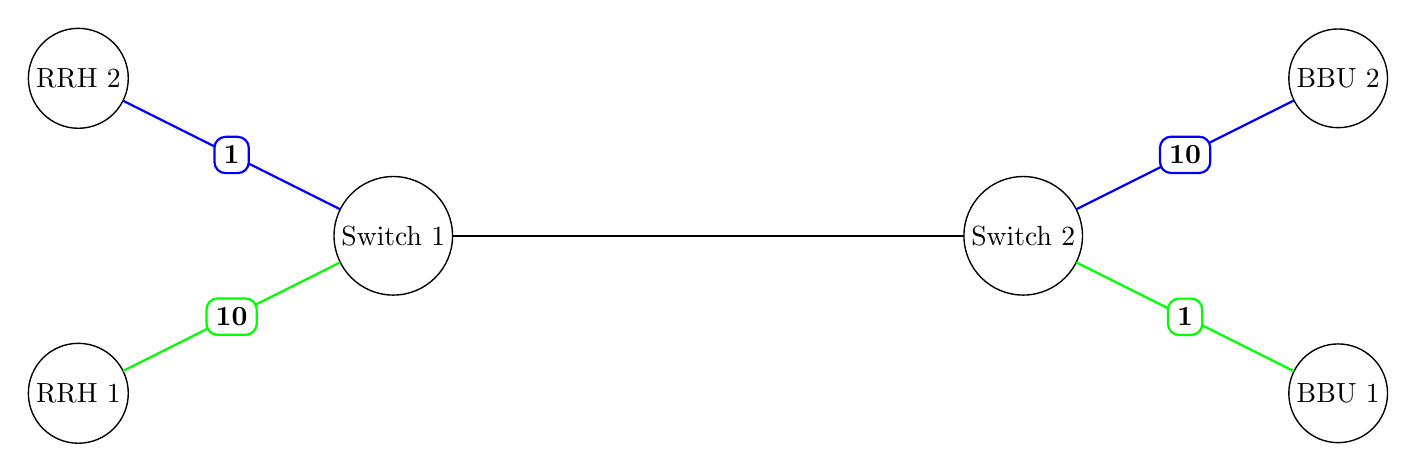
\begin{tikzpicture}
  \SetGraphUnit{5}
  \Vertex[x=0,y=0]{RRH 1}
  \Vertex[x=0,y=4]{RRH 2}

  
  \Vertex[x=16,y=0]{BBU 1}
  \Vertex[x=16,y=4]{BBU 2}

  \Vertex[x=4,y=2]{Switch 1}
  \Vertex[x=12,y=2]{Switch 2}
  

  \tikzset{
  EdgeStyle/.append style = {green} }
  \Edge[label = 1](BBU 1)(Switch 2)
  \Edge[label = 10](Switch 1)(RRH 1)
  
  \tikzset{
  EdgeStyle/.append style = {blue} }
  \Edge[label = 10](BBU 2)(Switch 2)
  \Edge[label = 1](Switch 1)(RRH 2)
  
  
  \tikzset{
  EdgeStyle/.append style = {black} }
  \Edge(Switch 1)(Switch 2)
\end{tikzpicture}
  }

  
\end{frame}


\begin{frame}{No waiting times}

  \centering
  \scalebox{0.65}{
  
\begin{tikzpicture}
  \SetGraphUnit{5}

  
  \node (0) at (1,-1){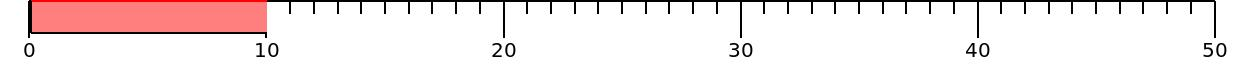
\includegraphics[scale=0.1]{chronogrames/10.jpeg}};
  \node (1) at (1,5){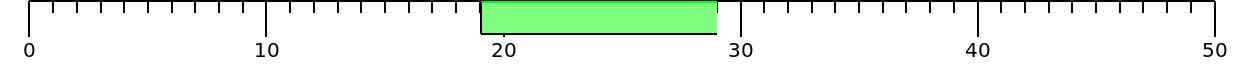
\includegraphics[scale=0.1]{chronogrames/11.jpeg}};
  \node (2) at (5,2){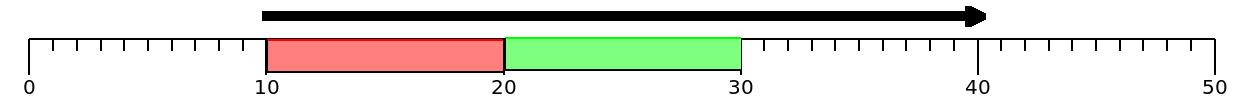
\includegraphics[scale=0.1]{chronogrames/12.jpeg}};
  \node (3) at (10,2){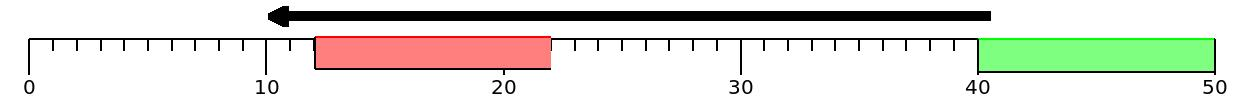
\includegraphics[scale=0.1]{chronogrames/15.jpeg}};
  \node (4) at (15,-1){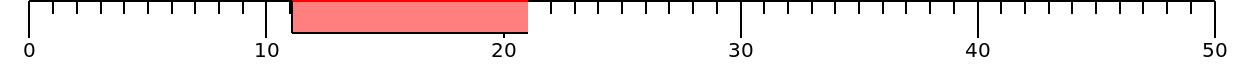
\includegraphics[scale=0.1]{chronogrames/13.jpeg}};
  \node (5) at (15,5){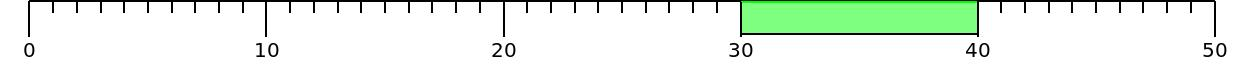
\includegraphics[scale=0.1]{chronogrames/14.jpeg}};
  
    \Edge(0)(2)
    \Edge(1)(2)
    \Edge(2)(3)
    \Edge(3)(4)
    \Edge(3)(5)
\end{tikzpicture}
  }
  
  
  With waiting times: 20(2k) / Without: 38(2k + 18)
  
\end{frame}




\begin{frame}{Heuristic}

   \centering
  \scalebox{0.5}{
  
\begin{tikzpicture}
  \SetGraphUnit{5}
  \Vertex[x=0,y=0]{RRH 3}
  \Vertex[x=0,y=4]{RRH 2}
  \Vertex[x=0,y=8]{RRH 1}
  
  \Vertex[x=16,y=0]{BBU 3}
  \Vertex[x=16,y=4]{BBU 2}
  \Vertex[x=16,y=8]{BBU 1}
  
  \Vertex[x=4,y=4]{Switch 1}
  \Vertex[x=12,y=4]{Switch 2}
  
  
  \tikzset{
  EdgeStyle/.append style = {green} }
  \Edge[label = $a_1$](BBU 1)(Switch 2)
  \Edge[label = 0](Switch 1)(RRH 1)
  
  \tikzset{
  EdgeStyle/.append style = {blue} }
  \Edge[label = $a_2$](BBU 2)(Switch 2)
  \Edge[label = 0](Switch 1)(RRH 2)
  
  \tikzset{
  EdgeStyle/.append style = {red} }
  \Edge[label = $a_3$](BBU 3)(Switch 2)
  \Edge[label = 0](Switch 1)(RRH 3)
  
  \tikzset{
  EdgeStyle/.append style = {black} }
  \Edge(Switch 1)(Switch 2)
\end{tikzpicture}
  
  }
  
  \begin{itemize}
  \item No waiting times on the longest route
  \item No route will have $T_i > T_j$ (j is the longer route)
  \end{itemize}

\end{frame}

\begin{frame}{Limits}
    
  \centering
  \scalebox{0.5}
  {
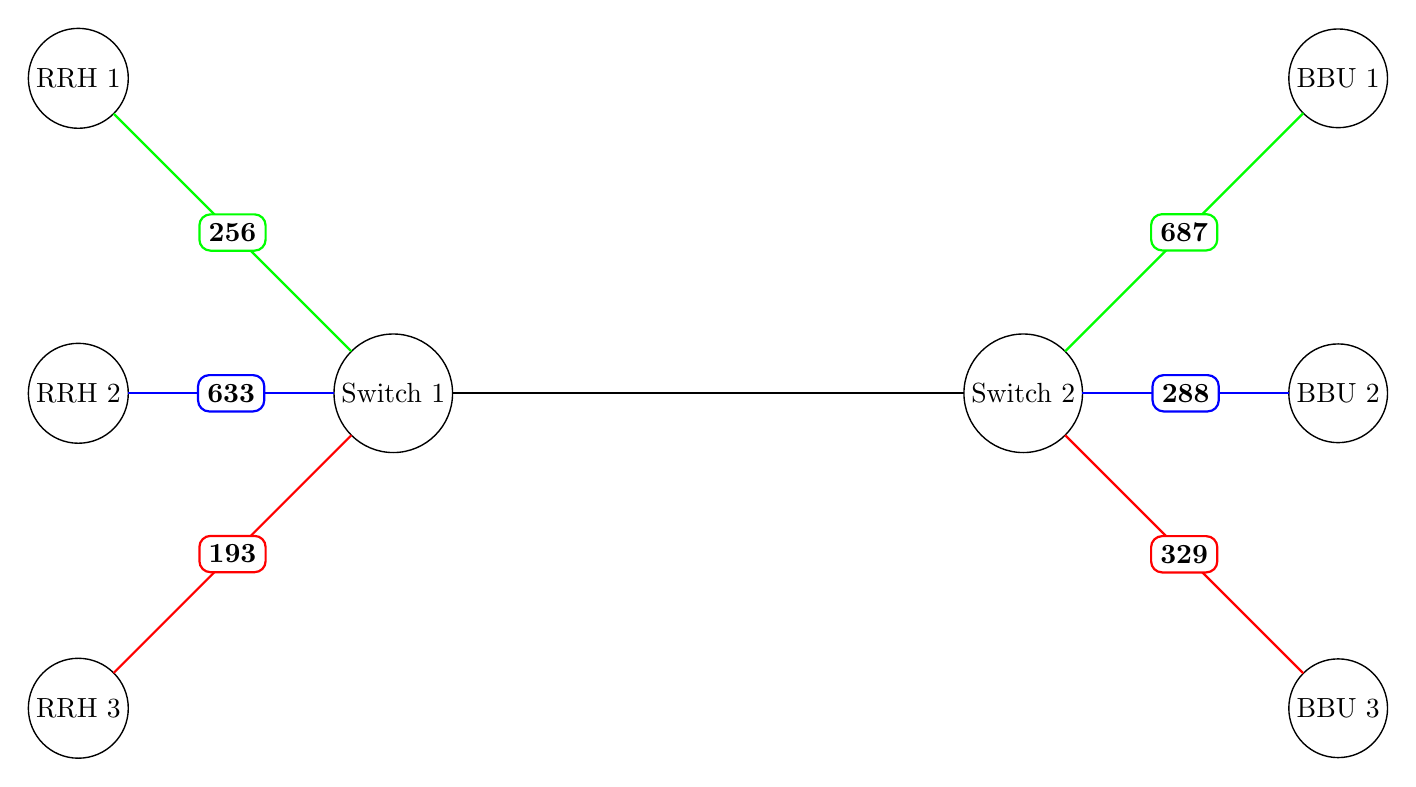
\begin{tikzpicture}
  \SetGraphUnit{5}
  \Vertex[x=0,y=0]{RRH 3}
  \Vertex[x=0,y=4]{RRH 2}
  \Vertex[x=0,y=8]{RRH 1}
  
  \Vertex[x=16,y=0]{BBU 3}
  \Vertex[x=16,y=4]{BBU 2}
  \Vertex[x=16,y=8]{BBU 1}
  
  \Vertex[x=4,y=4]{Switch 1}
  \Vertex[x=12,y=4]{Switch 2}
    
  \tikzset{
  EdgeStyle/.append style = {green} }
  \Edge[label = 687](BBU 1)(Switch 2)
  \Edge[label = 256](Switch 1)(RRH 1)
  
  \tikzset{
  EdgeStyle/.append style = {blue} }
  \Edge[label = 288](BBU 2)(Switch 2)
  \Edge[label = 633](Switch 1)(RRH 2)
  
  \tikzset{
  EdgeStyle/.append style = {red} }
  \Edge[label = 329](BBU 3)(Switch 2)
  \Edge[label = 193](Switch 1)(RRH 3)
  
  \tikzset{
  EdgeStyle/.append style = {black} }
  \Edge(Switch 1)(Switch 2)
\end{tikzpicture}

  }
  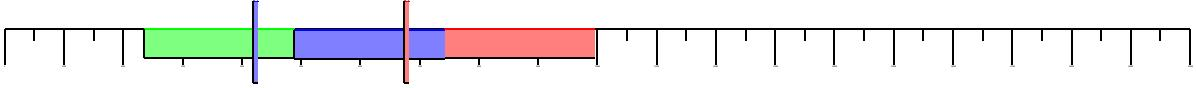
\includegraphics[scale = 0.2]{chronogrames/16.jpeg}
  
  $T_{max}$ = 4022 slots - Longest route delay *2 = 3268
  
  Optimal by splitting the emissions
\end{frame}



\begin{frame}{Conclusion}
\setbeamertemplate{blocks}[rounded]%
[shadow = true]
\begin{block}{Good results}
Heuristic giving optimal solutions on single cases, and good solution on hardest cases.
\end{block}
\begin{block}{Np-Hardness}
Similar problems proven Np-Hard.
\end{block}
\begin{block}{Approximations}
Algorithms trying to find optimal solutions in given periods.
\end{block}
\begin{block}{``Smart Bruteforce''}
Algorithm branch and bound to find an optimal solution, if it exists in a given period.
\end{block}

\end{frame}

\end{document}
